% =============================================================================
% COPYRIGHT AND DISCLAIMER
% =============================================================================
% This file is provided as a convenience template for competition participants.
% By using it, you accept full responsibility for compliance with all applicable
% copyright, licensing, and usage rules of the Association for Computing
% Machinery (ACM) and of any LaTeX packages you load (including, without
% limitation, the "acmart" document class and related ACM materials).
%
% Consult ACM's official publication, template, and copyright policies before
% using this setup for any purpose other than this competition. Do not assume
% that this template may be reused, redistributed, or submitted elsewhere
% without independently verifying ACM's current rules.
%
% Use of the "acmart" class, the "sigconf" option, or ACM-style formatting in
% this template does NOT mean that this report, this competition, its organizers,
% or any resulting PDF is sponsored, endorsed, affiliated with, or published by
% ACM. ACM trademarks and branding remain the property of ACM.
%
% Template packages live in preamble.tex.
% Citations live in main.bib. Edit this file with your paper content.
% =============================================================================
%
% Our report, written in the official template of the competition (read-only Overleaf project linked on
% the competition's "Final Submission" page): preamble.tex and the black template text are unchanged, the
% gray guide text is replaced by our content. Figures are read from docs/figures.
% Build: python docs/report/build_pdf.py --out build/

\documentclass[sigconf]{acmart}
% =============================================================================
% Template setup — participants normally do not edit this file.
% Author content belongs in main.tex; citations belong in main.bib.
% \documentclass lives in main.tex so Overleaf does not treat this file as root.
% =============================================================================

% --- Competition / non-ACM-submission friendly rights metadata -------------
\setcopyright{none}
\settopmatter{printacmref=false}
\acmConference[Kaggle Competition]{Filament Segmentation Challenge}{2026}{\href{https://www.kaggle.com/competitions/filament-segmentation-2026}{kaggle.com/competitions/filament-segmentation-2026}}
\acmBooktitle{Competition Report}
\acmDOI{}
\acmISBN{}

% --- Author guidance text --------------------------------------------------
% \guide{...} is gray italic while \guideStyletrue; omitted from the PDF if false.
% Flip the switch in main.tex after % =============================================================================
% Template setup — participants normally do not edit this file.
% Author content belongs in main.tex; citations belong in main.bib.
% \documentclass lives in main.tex so Overleaf does not treat this file as root.
% =============================================================================

% --- Competition / non-ACM-submission friendly rights metadata -------------
\setcopyright{none}
\settopmatter{printacmref=false}
\acmConference[Kaggle Competition]{Filament Segmentation Challenge}{2026}{\href{https://www.kaggle.com/competitions/filament-segmentation-2026}{kaggle.com/competitions/filament-segmentation-2026}}
\acmBooktitle{Competition Report}
\acmDOI{}
\acmISBN{}

% --- Author guidance text --------------------------------------------------
% \guide{...} is gray italic while \guideStyletrue; omitted from the PDF if false.
% Flip the switch in main.tex after % =============================================================================
% Template setup — participants normally do not edit this file.
% Author content belongs in main.tex; citations belong in main.bib.
% \documentclass lives in main.tex so Overleaf does not treat this file as root.
% =============================================================================

% --- Competition / non-ACM-submission friendly rights metadata -------------
\setcopyright{none}
\settopmatter{printacmref=false}
\acmConference[Kaggle Competition]{Filament Segmentation Challenge}{2026}{\href{https://www.kaggle.com/competitions/filament-segmentation-2026}{kaggle.com/competitions/filament-segmentation-2026}}
\acmBooktitle{Competition Report}
\acmDOI{}
\acmISBN{}

% --- Author guidance text --------------------------------------------------
% \guide{...} is gray italic while \guideStyletrue; omitted from the PDF if false.
% Flip the switch in main.tex after \input{preamble}.
%
% Do not use \guide{...} for \email{...}.
\usepackage{xcolor}
\newif\ifguideStyle
\guideStyletrue
\newcommand{\guide}[1]{%
  \ifguideStyle
    {\color{gray!65}\itshape #1}%
  \fi
}

% --- Math ------------------------------------------------------------------
% Do NOT load amssymb (or amsfonts): acmart already loads newtxmath, which
% defines the same symbols (e.g. \Bbbk) and causes a conflict on Overleaf.
% amsmath is already provided by acmart; mathtools extends it.
\usepackage{mathtools}

% --- Figures ---------------------------------------------------------------
% graphicx is already loaded by acmart
\usepackage{subcaption}

% --- Tables ----------------------------------------------------------------
% booktabs is already loaded by acmart
\usepackage{tabularx}
\usepackage{multirow}

% --- Bibliography style is set in main.tex (ACM-Reference-Format) ----------
.
%
% Do not use \guide{...} for \email{...}.
\usepackage{xcolor}
\newif\ifguideStyle
\guideStyletrue
\newcommand{\guide}[1]{%
  \ifguideStyle
    {\color{gray!65}\itshape #1}%
  \fi
}

% --- Math ------------------------------------------------------------------
% Do NOT load amssymb (or amsfonts): acmart already loads newtxmath, which
% defines the same symbols (e.g. \Bbbk) and causes a conflict on Overleaf.
% amsmath is already provided by acmart; mathtools extends it.
\usepackage{mathtools}

% --- Figures ---------------------------------------------------------------
% graphicx is already loaded by acmart
\usepackage{subcaption}

% --- Tables ----------------------------------------------------------------
% booktabs is already loaded by acmart
\usepackage{tabularx}
\usepackage{multirow}

% --- Bibliography style is set in main.tex (ACM-Reference-Format) ----------
.
%
% Do not use \guide{...} for \email{...}.
\usepackage{xcolor}
\newif\ifguideStyle
\guideStyletrue
\newcommand{\guide}[1]{%
  \ifguideStyle
    {\color{gray!65}\itshape #1}%
  \fi
}

% --- Math ------------------------------------------------------------------
% Do NOT load amssymb (or amsfonts): acmart already loads newtxmath, which
% defines the same symbols (e.g. \Bbbk) and causes a conflict on Overleaf.
% amsmath is already provided by acmart; mathtools extends it.
\usepackage{mathtools}

% --- Figures ---------------------------------------------------------------
% graphicx is already loaded by acmart
\usepackage{subcaption}

% --- Tables ----------------------------------------------------------------
% booktabs is already loaded by acmart
\usepackage{tabularx}
\usepackage{multirow}

% --- Bibliography style is set in main.tex (ACM-Reference-Format) ----------

\graphicspath{{../figures/}}

% Guide styling: \guideStyletrue = show gray italic hints; \guideStylefalse = omit them
% \guideStyletrue
\guideStylefalse

\begin{document}

\title{Consensus-Trained Full-Resolution U-Nets with PQ-Aware Instance Selection}
\subtitle{A Solution to the Solar Filament Segmentation Challenge 2026} % DO NOT CHANGE

% Author block: the repository keeps these placeholders (no personal data); build_pdf.py fills them in its
% build copy (--author, --institution, --city, --country, --email)
\author{[Author name]}
\affiliation{%
  \institution{[Institution (optional)]}
  \city{[City]}
  \country{[Country]}
}
\email{[e-mail]}

\begin{abstract}
    This report describes our solution to the Solar Filament Segmentation Challenge~2026, a Kaggle competition on automatic segmentation of solar filaments in GONG H-$\alpha$ observations. Two experts annotating the same image agree at a Panoptic Quality (PQ) of only 0.34, so annotator style dominates the metric. We train U-Nets at the native $2048\times2048$ resolution on the soft consensus of all annotators, take connected components as instances, and select instances with an exact per-component decomposition of PQ: the post-processing is chosen by nested cross-validation and the final keep decision is made by a small learned component filter. Ten networks (ResNet34 and EfficientNetV2-S encoders, five folds each) reach a nested out-of-fold PQ of 0.447 (95\,\% interval 0.438--0.457) at about 8\,s per image on one T4 GPU; five networks reach 0.444 at about 5\,s. Code, weights and a notebook that reproduces both submissions without re-training are available at \href{https://github.com/WLHsu0827/ieee-bigdata26-filament}{github.com/WLHsu0827/ieee-bigdata26-filament}.
\end{abstract}

\maketitle


% ==================================== %
%              INTRODUCTION            %
% ==================================== %
\section{Introduction}
    This report goes over the details of our submitted solution to the Solar Filament Segmentation Challenge~2026 \cite{filament-segmentation-2026}. The challenge, launched on July~10,~2026, is organized by the Earth-Space AI Research (ESAIR) Lab\footnote{\href{https://www.esairlab.com/home}{www.esairlab.com/}}. This challenge utilizes the MAGFiLO dataset for evaluation of the segmentation algorithms \cite{ahmadzadeh2024dataset}. Predictions are ranked by PQ \cite{kirillov2019panoptic}: a predicted and an annotated filament match if their intersection over union (IoU) exceeds 0.5, $\mathrm{PQ}=\sum_{\mathrm{TP}}\mathrm{IoU}/(|\mathrm{TP}|+\tfrac12|\mathrm{FP}|+\tfrac12|\mathrm{FN}|)$, and every annotator's set of filaments is scored separately, with the counts pooled over the test set. Our solution has four parts: a label analysis that sets realistic targets, U-Nets trained at native resolution on the annotators' consensus, an exact decomposition of PQ over predicted components that makes nested cross-validation of the post-processing cheap, and a learned PQ-aware component filter that needs only numpy at inference.


% ==================================== %
%              METHODOLOGY             %
% ==================================== %
\section{Methodology}\label{sec:methodology}

\subsection{Data, labels and splits}
The 707 training observations come from six GONG \cite{harvey1996gong} sites (2011--2022) with 1,154 annotator sets and 8,199 filament polygons (411 images with one annotator, 145 with two, 151 with three); the 180 test observations are used only for the submissions. Two properties of the labels shape the method. \emph{Instances do not touch:} the 8,199 polygons form 8,219 connected components of their per-annotator unions, so instance segmentation reduces to semantic segmentation followed by connected components. \emph{Annotators disagree:} one annotator scored against another reaches PQ 0.340 (SQ 0.634, RQ 0.536) on the 296 multi-annotator images, the union or intersection of two annotators predicts a third no better (0.332 / 0.314), and an oracle that outputs the consensus of all annotators, including the scored one, reaches 0.648. A model can therefore at best predict what annotators agree on.

All models use the same five folds of the training images (142, 142, 141, 141 and 141 images), grouped by image so that all annotators of an image fall into one fold. Each network is trained on four folds and predicts the fifth; these out-of-fold maps of all 707 images are the only data for every post-processing choice and every evaluation (\S\ref{sec:evaluation}), and every choice is validated by nested cross-validation over the same folds.

\begin{figure*}[t]
  \centering
  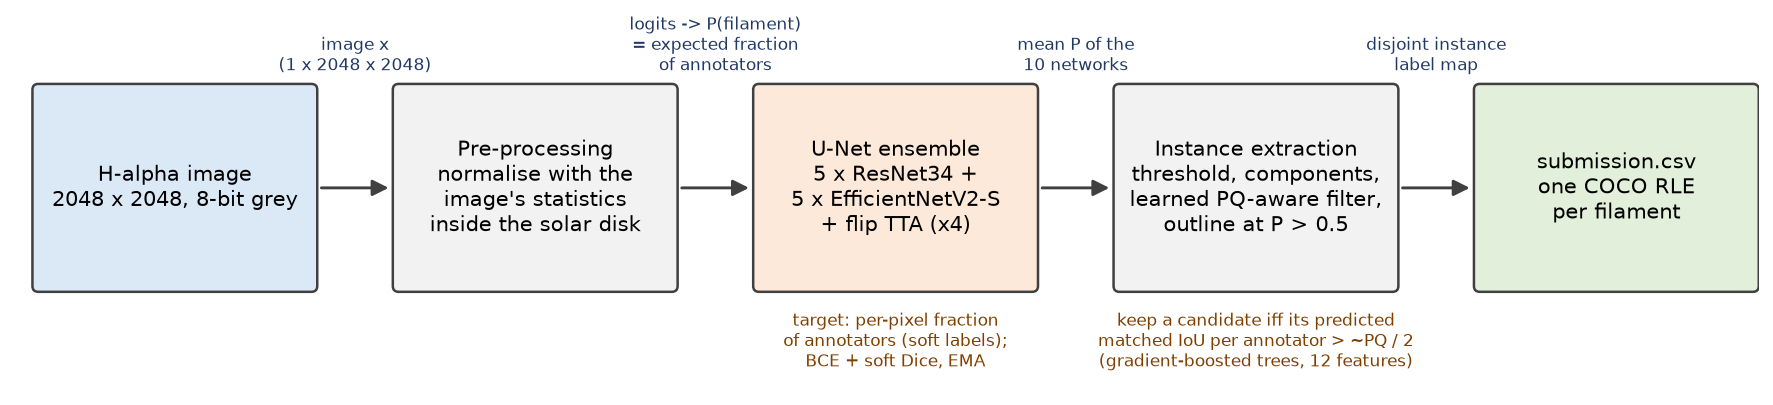
\includegraphics[width=\textwidth]{pipeline.png}
  \caption{End-to-end pipeline: inputs, processing blocks and the key intermediate signals.}
  \Description{Block diagram: the H-alpha image is normalised inside the solar disk, ten U-Nets with flip test-time augmentation are averaged into a probability map, instances are extracted and filtered by a learned PQ-aware filter, and the submission file holds one RLE mask per filament.}
  \label{fig:pipeline}
\end{figure*}

\subsection{Pipeline and networks}
\emph{Pre-processing and target.} Fig.~\ref{fig:pipeline} summarises the end-to-end pipeline. The input is one grey channel at full resolution, normalised by the mean and standard deviation of the pixels inside the solar disk, which removes exposure differences between sites. The training target is the soft consensus: the fraction of an image's annotators that draw each pixel, so the network output estimates the probability that an annotator draws the pixel.

\emph{Networks.} U-Net \cite{ronneberger2015unet}, an encoder--decoder with skip connections at every scale (segmentation-models-pytorch \cite{smp}), with an ImageNet-pretrained ResNet34 \cite{he2016resnet} or EfficientNetV2-S \cite{tan2021efficientnetv2,timm} encoder and one output channel.

\emph{Sampling and training.} Every epoch draws four $768\times768$ crops per training image from the 2048\,px image, centred (up to a random shift of a quarter crop) on a random filament pixel with probability 0.7 and on a random pixel otherwise; a 1.6 times larger window is rotated by an arbitrary angle, scaled by 0.9--1.1, flipped and centre-cropped, followed by gamma, contrast, blur and noise jitter. Loss: binary cross-entropy plus soft Dice; AdamW (learning rate $3\cdot10^{-4}$, weight decay $10^{-4}$), linear warm-up and cosine decay, mixed precision and an exponential moving average of the weights (decay 0.999 with warm-up); 30 epochs (ResNet34) or a 1.5\,h budget per fold (EfficientNetV2-S, 21--24 epochs) on one T4 GPU.

\emph{Inference.} Each network predicts the full image with flip test-time augmentation ($\times4$) and the ten networks are averaged. Since both encoders share the folds, the out-of-fold map of a training image averages only the two networks that did not see it, so the selection is transferred from two-network to ten-network averages. On the test images this transfer is benign: with the same selection the ten-network average keeps 3--4\,\% fewer instances than the five two-network averages, inside their fold-to-fold range, and agrees with each of them at a PQ of 0.91, more than two-network selections of different folds agree with each other (0.87).

% Floats are defined here, ahead of their first reference, so that LaTeX places them next to it: Fig. 2 and
% Table 1 at the tops of the two columns of page 2, the full-width Fig. 3 at the top of page 3 above Sec. 3.
\begin{figure}[t]
  \centering
  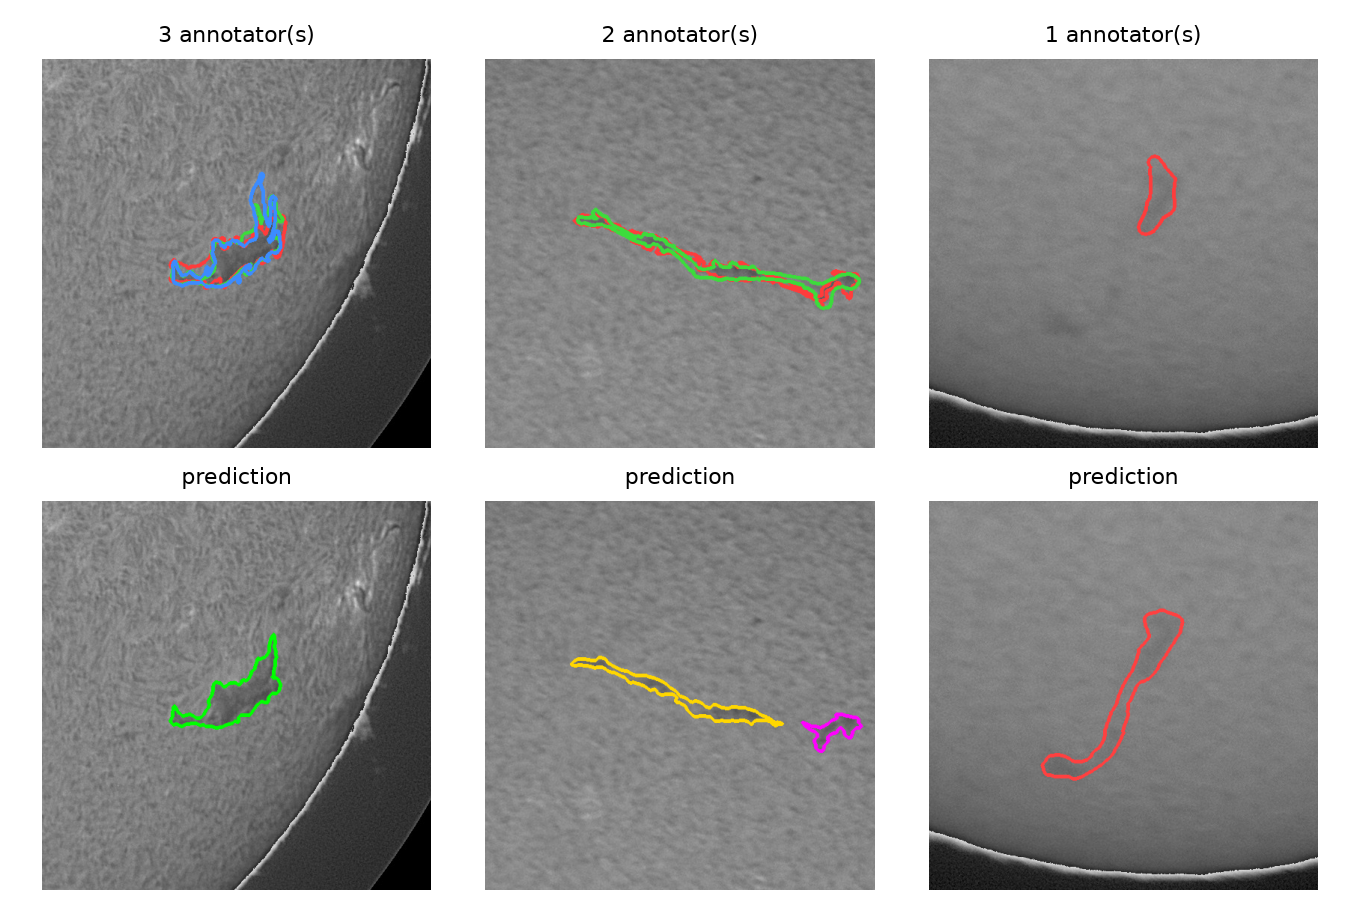
\includegraphics[width=\columnwidth]{morphology.png}
  \caption{Validation examples (fold 0, final configuration). Top: annotator outlines (one colour per annotator); bottom: predicted instances. Left: a match; middle: a filament chain predicted as two instances; right: the prediction follows a faint filament beyond the single annotator's outline.}
  \Description{Six zoomed panels of H-alpha images: three with annotator outlines on top and the corresponding predicted filament instances below.}
  \label{fig:morph}
\end{figure}

\begin{table}[t]
  \caption{PQ of the main models: fold 0, or mean $\pm$ standard deviation over the five folds, with one fixed rule; nested cross-validation over all 707 out-of-fold images with 95\,\% bootstrap intervals; public leaderboard (LB, about 90 test images).}
  \label{tab:results}
  \small
  \setlength{\tabcolsep}{2.4pt}
  \begin{tabular}{lccc}
    \toprule
    model & fixed rule & nested & LB\\
    \midrule
    classical darkness threshold & 0.092$^a$ & -- & 0.07\\
    U-Net R34, 512\,px full disk & 0.365$^a$ & -- & 0.30\\
    U-Net R34, 1024\,px full disk & 0.416$^a$ & 0.425$^b$ & 0.35\\
    U-Net R34, 2048\,px & 0.422\,$\pm$\,0.005 & 0.432 & --\\
    U-Net EffV2-S, 2048\,px & 0.432\,$\pm$\,0.007 & 0.440 & --\\
    \quad + learned filter (\emph{fast}) & -- & 0.444 & 0.38\\
    10 networks, rule (A)$^c$ & -- & 0.443 {\footnotesize[.434, .453]} & 0.39\\
    \quad + learned filter (B) & -- & \textbf{0.447} {\footnotesize[.438, .457]} & 0.38\\
    \midrule
    annotator vs.\ annotator & \multicolumn{2}{c}{0.340} & --\\
    \bottomrule
  \end{tabular}\\[2pt]
  {\footnotesize $^a$fold 0. $^b$nested over five sub-folds of fold 0. $^c$robust objective $r=0.77$ (plain PQ: nested 0.442, LB 0.38).\par}
\end{table}

\begin{figure*}[t]
  \centering
  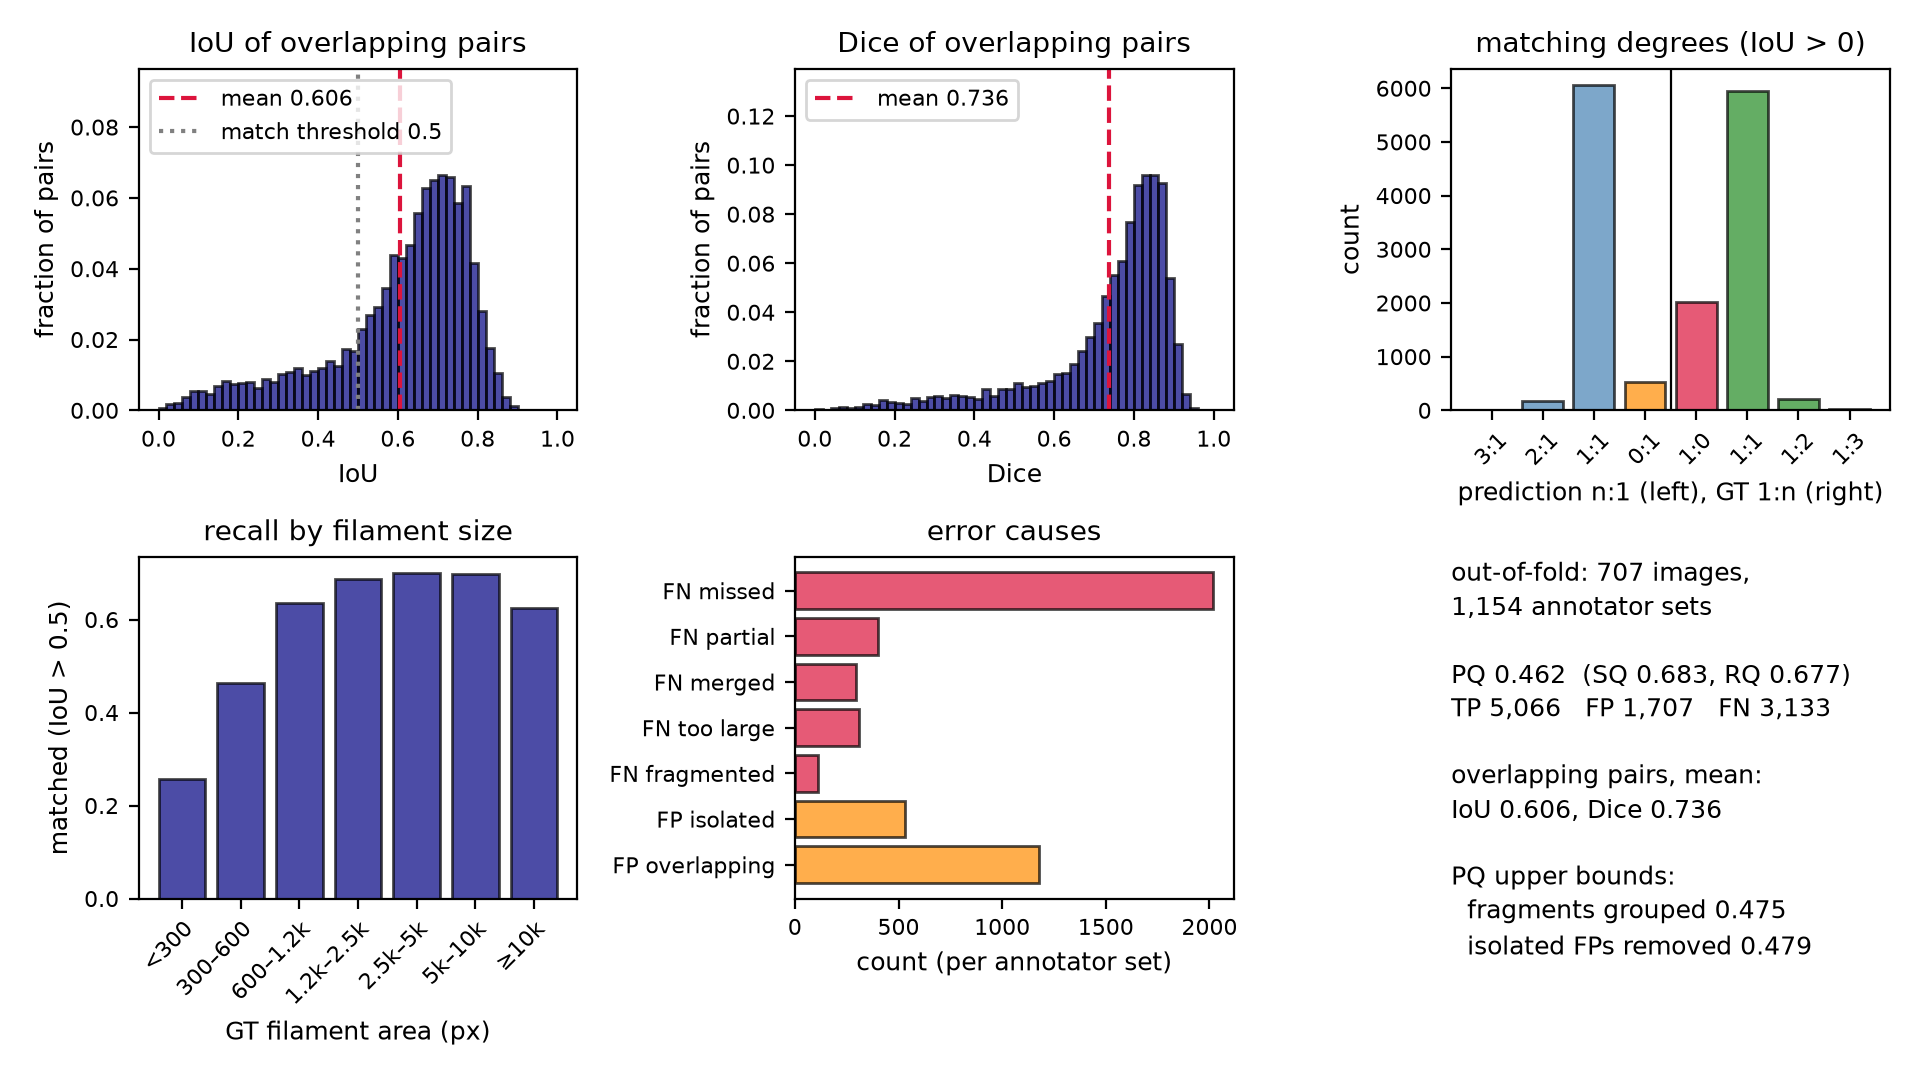
\includegraphics[width=\textwidth]{evaluation_grid.png}
  \caption{Evaluation of the final configuration on the out-of-fold maps of all 707 training images (1,154 annotator sets); the learned filter was fitted on these maps, so PQ 0.462 is optimistic (nested estimate 0.447, Table~\ref{tab:results}). Top: IoU and Dice of overlapping predicted and annotated filaments, and matching degrees: how many predictions overlap an annotated filament (1:$n$; 1:0 = missed) and how many annotated filaments overlap a prediction ($n$:1; 0:1 = spurious). Bottom: recall by filament area (error bars and the PQ interval in the text panel: 95\,\% bootstrap intervals over images, 2,000 resamples) and the cause of every error. Unmatched filaments are \emph{missed} (no overlapping prediction), \emph{partial} (the best prediction covers less than half), \emph{merged} with a neighbour, inside a prediction that is \emph{too large}, or \emph{fragmented} (the union of several predictions would match); false positives are \emph{isolated} or \emph{overlap} a filament with IoU $\le0.5$. Upper bounds: PQ if each annotator's fragments were grouped or all isolated false positives removed.}
  \Description{Six panels: histograms of IoU and Dice of overlapping pairs, bar charts of matching degrees, recall by filament size and error causes, and a text panel with the summary numbers.}
  \label{fig:eval}
\end{figure*}

\subsection{Instances and an exact decomposition of PQ}
Instances are the 8-connected components of the thresholded map after hole filling. Because predicted instances are disjoint, a component $c$ matches at most one filament per annotator set, and with $v_c=\sum_{e\in E(c)}\mathrm{IoU}_e(c)\,[\mathrm{IoU}_e(c)>0.5]$ over the $|E(c)|$ annotator sets of its image,
\begin{equation}
\mathrm{PQ}(K)=\frac{\sum_{c\in K}v_c}{\tfrac12\sum_{c\in K}|E(c)|+\tfrac12 G}
\end{equation}
for a kept set $K$ and $G$ annotated filaments. Keeping $c$ improves PQ iff $v_c/|E(c)|>\mathrm{PQ}/2$: at PQ $\approx0.45$ a candidate is worth keeping if it has roughly a 33\,\% chance of matching an annotator. Candidate components and their $v_c$ are computed once per \emph{shape} (detection threshold, closing, outline level); any \emph{selection} is then scored exactly and instantly, which makes nested cross-validation of the post-processing cheap (unit-tested against the official code).

\subsection{Selection and learned component filter}
The shape and a rule (minimum area, mean and peak probability) are chosen by nested cross-validation on the 707 out-of-fold maps: for each outer fold the best choice on the other four folds is applied to it, and the pooled counts give an unbiased estimate. Detection and extent are decoupled: components are detected at a low threshold (0.25), and each kept instance is redrawn where the probability exceeds 0.5. As objective we use plain PQ and a robust variant that assumes each filament is labelled only with probability $r$, $\mathrm{PQ}_r=rS/(r\,\mathrm{TP}+\tfrac12\mathrm{FP}+\tfrac12(1-r)\mathrm{TP}+\tfrac12 r\,\mathrm{FN})$ with $S$ the summed IoU of the matches, which penalises marginal detections more ($r=0.77$). The rule of our final submission~A keeps components with mean probability $\ge0.85$ and peak $\ge0.99$.

In our final submission~B the keep decision is made by gradient-boosted regression trees (200 trees, at most 15 leaves) that predict $v_c/|E(c)|$ from 12 features of each candidate: log area, mean, peak, 90th percentile and standard deviation of the probability, elongation, length, width, bounding-box fill ratio, distance from the disk centre, number of candidates in the image and area rank. A candidate is kept if its prediction exceeds a threshold chosen on grouped out-of-fold predictions (0.28). The trees are exported to JSON, so inference needs only numpy. Fig.~\ref{fig:morph} shows segmentations of validation images.

% ==================================== %
%              EVALUATION              %
% ==================================== %
\section{Evaluation}\label{sec:evaluation}
\emph{Strategy.} Our implementation of PQ follows the organisers' self-evaluation notebook (identical scores) and pools the counts over all 1,154 annotator sets of the 707 out-of-fold maps, as the leaderboard does over the test set. Every post-processing choice is estimated by nested cross-validation (\S\ref{sec:methodology}). Uncertainty is reported as the standard deviation over the five folds, as 95\,\% bootstrap intervals over images (4,000 resamples) and, for comparisons, as paired bootstrap differences on the same images. The public leaderboard served only to check that choices transfer.

\emph{Results.} Table~\ref{tab:results} shows that native resolution matters ($+0.05$ from 512 to 1024\,px, $+0.01$ to 2048\,px) and that EfficientNetV2-S beats ResNet34 by 0.01 per fold. Combining both encoders adds 0.002 over five EfficientNetV2-S networks, and the learned filter adds 0.004 over the rule on the same maps (paired difference $+0.0038$, SD 0.0013, positive in 99.8\,\% of the resamples). The nested estimates vary between folds by an SD of 0.005 (A) and 0.006 (B); both final configurations are far above the agreement of two annotators (0.340).

\emph{Error analysis.} Fig.~\ref{fig:eval} shows the quantities used by the organisers. The final ensemble matches 62\,\% of the annotated filaments (SQ 0.68). On images with several annotators it matches 82\,\% of the filaments that another annotator also drew, but only 32\,\% of those drawn by a single annotator. Of the filaments without any overlapping prediction (25\,\%), 71\,\% are smaller than 1,200\,px and 74\,\% contain probabilities above 0.5---the network sees them, but keeping them would cost more false positives than it gains. Fragmentation and merging are rare: 2.8\,\% of the annotated filaments overlap two or more predictions and 2.6\,\% of the predictions overlap two or more filaments. Grouping each annotator's fragments separately would add at most 0.013 PQ, but one output must serve all annotators: an oracle that picks the best grouping of components across detection levels gains only 0.003 (fold 0), whereas an oracle choosing each component's outline would gain 0.012. The remaining errors are mostly faint, small or annotator-specific filaments and outlines that decide whether a match crosses IoU 0.5 (Fig.~\ref{fig:morph}).

\emph{Public leaderboard.} The public score is 0.82--0.88 of the nested validation score for every model although the models predict as many filaments per test image as per validation image; the gap is consistent with sparser test labels. Stricter selections never transferred worse: the nested rules beat the grid-tuned rule of the 1024\,px model (0.35 vs.\ 0.34), and for the ensemble the robust objective beat plain PQ (0.39 vs.\ 0.38). The learned filter's cross-validated gain did not show on the public part (0.38; 93\,\% of its instances are shared with the rule's submission, so the difference rests on a few dozen filaments of about 90 images; a score on 90 images scatters with SD 0.012 around the score on all images, estimated from random subsets of our out-of-fold images).

\emph{Efficiency and reproducibility.} Executing the pipeline notebook on one T4 GPU for the 180 test images takes 7.3--8.0\,s (ten networks, flip TTA $\times4$) plus about 0.5\,s (post-processing) per image in three runs; the \emph{fast} profile (five networks) takes 4.7--4.8\,+\,0.5\,s. From the stored fp16 weights one run of the notebook writes both final submissions, the learned filter's (public 0.38) and the rule's (0.39), from the same maps; they agree with the files built from the training-time predictions on 1,074 of 1,076 and 1,071 of 1,072 instances. Adding the four 90\textdegree{} rotations to the test-time augmentation ($\times8$) raises the nested out-of-fold PQ by only 0.001--0.003 for twice the network time, so the submission keeps $\times4$.

\emph{Strengths and weaknesses.} The method is simple (connected components are lossless here, so no instance head is needed), every reported number is a nested out-of-fold estimate with its uncertainty, and the exact decomposition turns post-processing into a cheap and honest selection problem; inference needs about 8\,s per image and only stored fp16 weights plus numpy for the filter. Its weaknesses mirror the labels: small and faint filaments (recall 26\,\% below 300\,px and 46\,\% at 300--600\,px) and filaments drawn by a single annotator are mostly dropped, outlines decide many matches near IoU 0.5, and ten networks cost more time than one.

\emph{What did not help.} (i) Noisy-student training \cite{xie2020noisystudent} with 1,200 unlabelled GONG archive images taken at least two days away from every competition image (listed with hashes in the repository), pseudo-labelled by the fold's own networks, did not help at equal compute (students 0.443 / 0.438 vs.\ teachers 0.445 / 0.442 on fold 0). (ii) Distance-based merging of nearby components, lower detection thresholds and global outline levels other than 0.5 were within noise. (iii) A larger encoder (EfficientNetV2-M) improved the fold-0 ensemble by 0.005--0.011, but not the ensemble on folds 0--2 ($-0.004$ to $+0.001$); extra weight on small filaments and their borders did not help either. A single-fold gate on 142 images is too noisy to decide. (iv) Choosing each candidate's outline level with a second regressor captured none of the 0.020 that an oracle would gain, and giving the filter each network's probabilities separately (+0.002) shifts between out-of-fold and submission ensembles, so neither was adopted.

\emph{Possible improvements.} As the remaining errors reflect annotator disagreement more than missed evidence, the most promising directions are an outline model trained on individual annotators' outlines, more labelled examples of faint and small filaments, and, for efficiency, distilling the ten networks into one (about 2\,s per image).



% ==================================== %
%            ACKNOWLEDGMENT            %
% ==================================== %
\section{Acknowledgment}\label{sec:acknowledgment}
    % Do not change
    The organization of the Filament Segmentation Challenge 2026 is partially supported by the U.S. National Science Foundation (NSF) under Grant No. 2209912 and 2433781, directorate for Computer and Information Science and Engineering (CSE), and Office of Advanced Cyberinfrastructure (OAC), and Grant No. 2511630, AST Division Of Astronomical Sciences and MPS Directorate for Mathematical and Physical Sciences.

    The Filament Segmentation Challenge 2026 is sponsored by the U.S. National Science Foundation (NSF) National Solar Observatory (NSO). 

    This work utilizes GONG data obtained by the NSO Integrated Synoptic Program, managed by the National Solar Observatory, which is operated by the Association of Universities for Research in Astronomy (AURA), Inc. under a cooperative agreement with the National Science Foundation and with contribution from the National Oceanic and Atmospheric Administration. The GONG network of instruments is hosted by the Big Bear Solar Observatory, High Altitude Observatory, Learmonth Solar Observatory, Udaipur Solar Observatory, Instituto de Astrofísica de Canarias, and Cerro Tololo Interamerican Observatory.

\bibliographystyle{ACM-Reference-Format}
\bibliography{main}

\end{document}
